\section{Einleitung}
In diesem Versuch soll die Relaxationszeit von Dipolen in Kristallen vermessen werden.



\section{Theorie der Dipole in Kristallgittern}
\label{sec:theorie}

Punkte eines Kristallgitters liegen auf einem regelmäßigen, drei dimensionalen Raster.
Die kleinste Einheit dieser Gitter ist die sogenannte Elementar- oder Einheitszelle.
Die Elementarzelle kann aus einem oder mehreren Punkten bzw.\ Atomen zusammengesetzt sein.
Die Gitterstruktur wird durch die gleichmäßige Fortsetzung der Elementarzelle in alle drei Raumrichtungen gebildet.
In einem Ionenkristall, wie das welches in diesem Versuch untersucht wird,
wird die Kristallstruktur durch die Ionenbindung zwischen zwei oder mehr Typen von Ionen gebildet.
Beispielsweise ordnet sich Cäsiumiodid zu einem kubisch-innenzentrierten Gitter an.
Die Wechselwirkung zwischen den Gitterpunkten erzeugt ein perdiodisches Potential,
welches die grundlegenden Eigenschaften,
wie zum Beispiel die Leitfähigkteit, des Festkörpers bestimmt.


\subsection{Dipole durch Leerstellen}

Durch Einbringung eines fremden Ions in den Kristall kann eine Leerstelle entstehen.
Dieser Gitterdefekt ändert zumindest lokal die Eigenschaften des Kristalls.
Das periodische Potential ist gegenüber dem reinen Kristall gestört.
So kann in Cäsiumiodid durch einbau eines Strontiumions $\ce{Sr++}$ eine Leerstelle im Gitter erzeugt werden.
Wie in \autoref{fig:leerstelle} dargestellt,
bildet sich ein Dipol zwischen der Leerstelle und dem Strontiumion.
Die Dipolachse der Störung zeigt dabei in Richtung einer der Translationsachsen des Kristalls.
Die Ausrichtung des Dipols kann sich durch sogenannte Leerstellendiffusion ändern.
\begin{figure}
  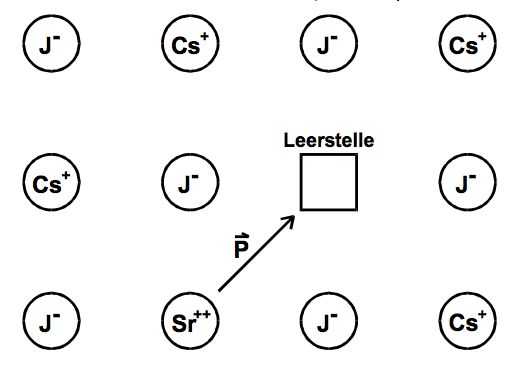
\includegraphics[width=0.8\textwidth]{pictures/leerstelle.png}
  \caption{Eine Leerstelle entsteht im Kristall durch einbringung von $\ce{Sr++}$ \cite{v48}. Dadurch entsteht ein Dipolmoment
  zwischen dem $\ce{Sr++}$ und der Leerstelle}
  \label{fig:leerstelle}
\end{figure}
Dafür muss Arbeit aufgebracht werden um das Gitterpotential an der Stelle zu überwinden.
Die thermische Energieverteilung der Dipole ist durch die Boltzmannstatistik nach \eqref{eq:boltzmann} vorgegeben.
Dabei ist $W$ die Arbeit, die verrichtet werden muss, damit die Leerstelle die Gitterstelle wechselt.
$T$ ist die Temperatur und $k_\text{B} = \SI{1,38064852e-23}{\joule \per \kelvin}$ die Boltzmannkonstante.
\begin{equation}
  E_D \propto \E^{- \frac{W}{k_\text{B} T}}
  \label{eq:boltzmann}
\end{equation}

Die Relaxationszeit, die Zeit nach der die Dipole ihre Orientierung wechseln,
beträgt im Mittel
\begin{equation}
  τ(T) = τ_0 \E^{\frac{W}{k_\text{B} T}}.
  \label{eq:time}
\end{equation}

Ziel dieses Versuches wird sein, die Aktivierungsenergie $W$ und die charackteristische Relaxationszeit $τ_0$ zu bestimmen.

\subsection{Dipole im äußeren elektrischen Feld }

Wird das dotierte Gitter einem elektrischen Feld ausgesetzt, so werden sich die Dipole,
soweit wie es die Gitterstruktur zulässt, in Feldlinienrichtung ausrichten.
Durch thermische Energie wird jedoch zu jeder Zeit ein Teil der Dipole die Ausrichtung ändern.
Der Anteil der in Feldrichtung ausgerichteten Dipole ist somit stochastisch bestimmt.
Dies ist die Grundlage für die Anwendbarkeit der Langevin-Formel~\eqref{eq:langevin}.
\begin{equation}
  \label{eq:langevin}
  L(x) = \coth(x) - \frac{1}{x}
\end{equation}
Diese beschreibt ursprünglich die Magnetisierung eines paramagnetischen Materials unter Einfluss eines äußeren Magnetfelds.
Die Langevin-Formel ist die klassische
Näherung der Brillouin-Formel~\eqref{eq:brillouin}.
Dabei ist
\begin{equation}
  x = \frac{\v{m}_B \v{B}}{k_\text{B} T},
\end{equation}
mit dem äußeren Magnetfeld $\v{B}$ und dem magnetischen Dipolmoment $\v{m}_B$.
Analog ist im Fall äußerer elektrische Felder, wie in diesem Versuch,
\begin{equation}
  x = \frac{\v{m} \v{E}}{k_\text{B} T}
\end{equation}
mit dem elektrischen Dipolmoment $\v{m}$ und dem externen elektrischen Feld $\v{E}$.
Bei richtiger Ausrichtung der elektrischen Feldlinien zu den Gittervektoren des Kristalls ist die Richtung des Dipolmoments im Mittel paralell zum elektrischen Feld.
Dann lässt sich die Langevin-Funktion parametrisieren mit
\begin{equation}
  x= \frac{m E}{k_\text{B} T}.
\end{equation}

\begin{equation}
  B_J(x) =   \frac{2J + 1}{2J} \coth\!\left( \frac{2J + 1}{2J} x \right)
           - \frac{1}{2J} \coth\!\left(\frac{1}{2J} x \right)
  \label{eq:brillouin}
\end{equation}


%
% \begin{figure}
%   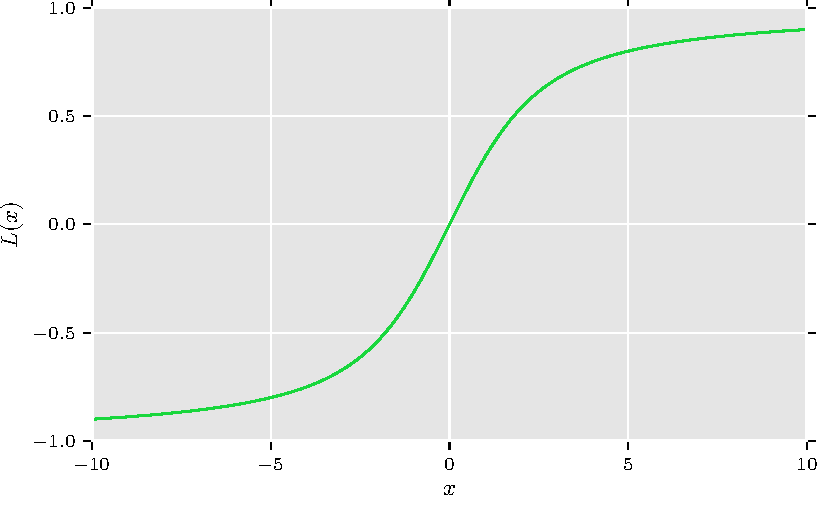
\includegraphics{langevin.pdf}
%   \caption{Langevin-Funktion im Bereich von \num{-10} bis \num{10}.}
%   \label{fig:langevin}
% \end{figure}


Im folgenden Versuchsaufbau ist $ x \ll 1 $. In diesem Bereich ist die Langevin Funktion annähernd Linear.
Dadurch kann die Näherung $L(x) \approx \frac{x}{3}$ genutzt werden.
Somit ergibt sich für den Anteil der zur Feldrichtung ausgerichteten Dipole

\begin{equation}
  L(T) \approx \frac{m E}{3 k_\text{B} T}.
  \label{eq:dipoles}
\end{equation}
